\chapter{Supplemental for Chapter \refchB}
%\counterwithin{figure}{section}
%\beginsupplement

\begin{figure}[H]
\centering
    %
    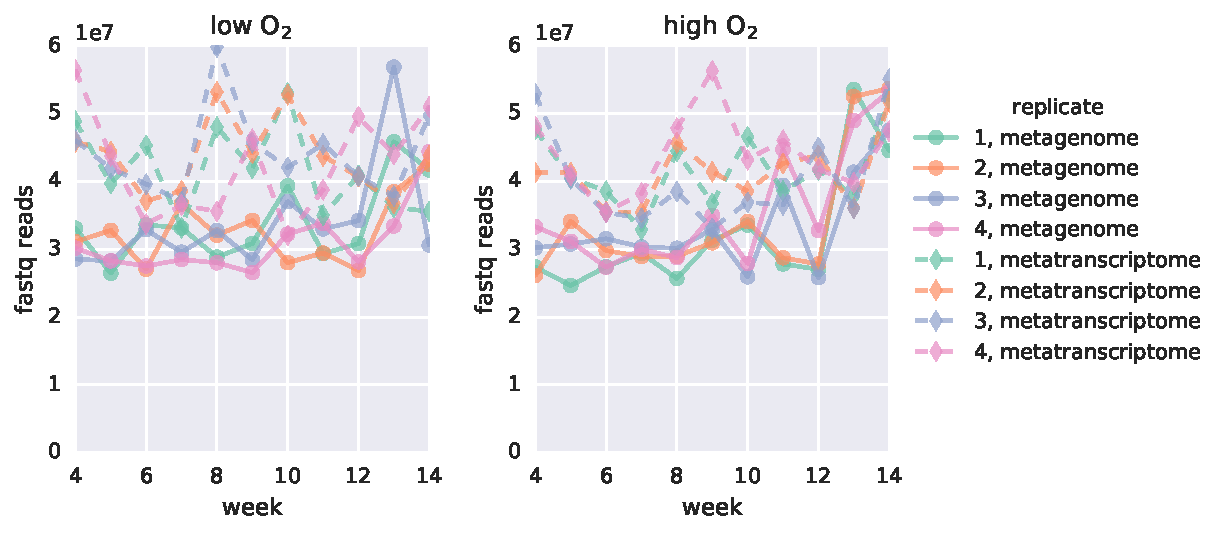
\includegraphics[width=1.0\textwidth]{./tex/chapter2/figures/170326_compare_raw_fastq_reads.pdf}
    \begin{singlespace}
    \caption[Number of reads in metagenomes and metatranscriptomes, by sample]{
        Number of reads in metagenomes and metatranscriptomes, by sample.}
    \label{fig:fastq_reads}
    \end{singlespace}
\end{figure}

\begin{figure}[H]
\centering
    % /Users/janet/Dropbox/thesis/tex/chapter2/figures/170314_mapping_fractions--portrait.pdf
    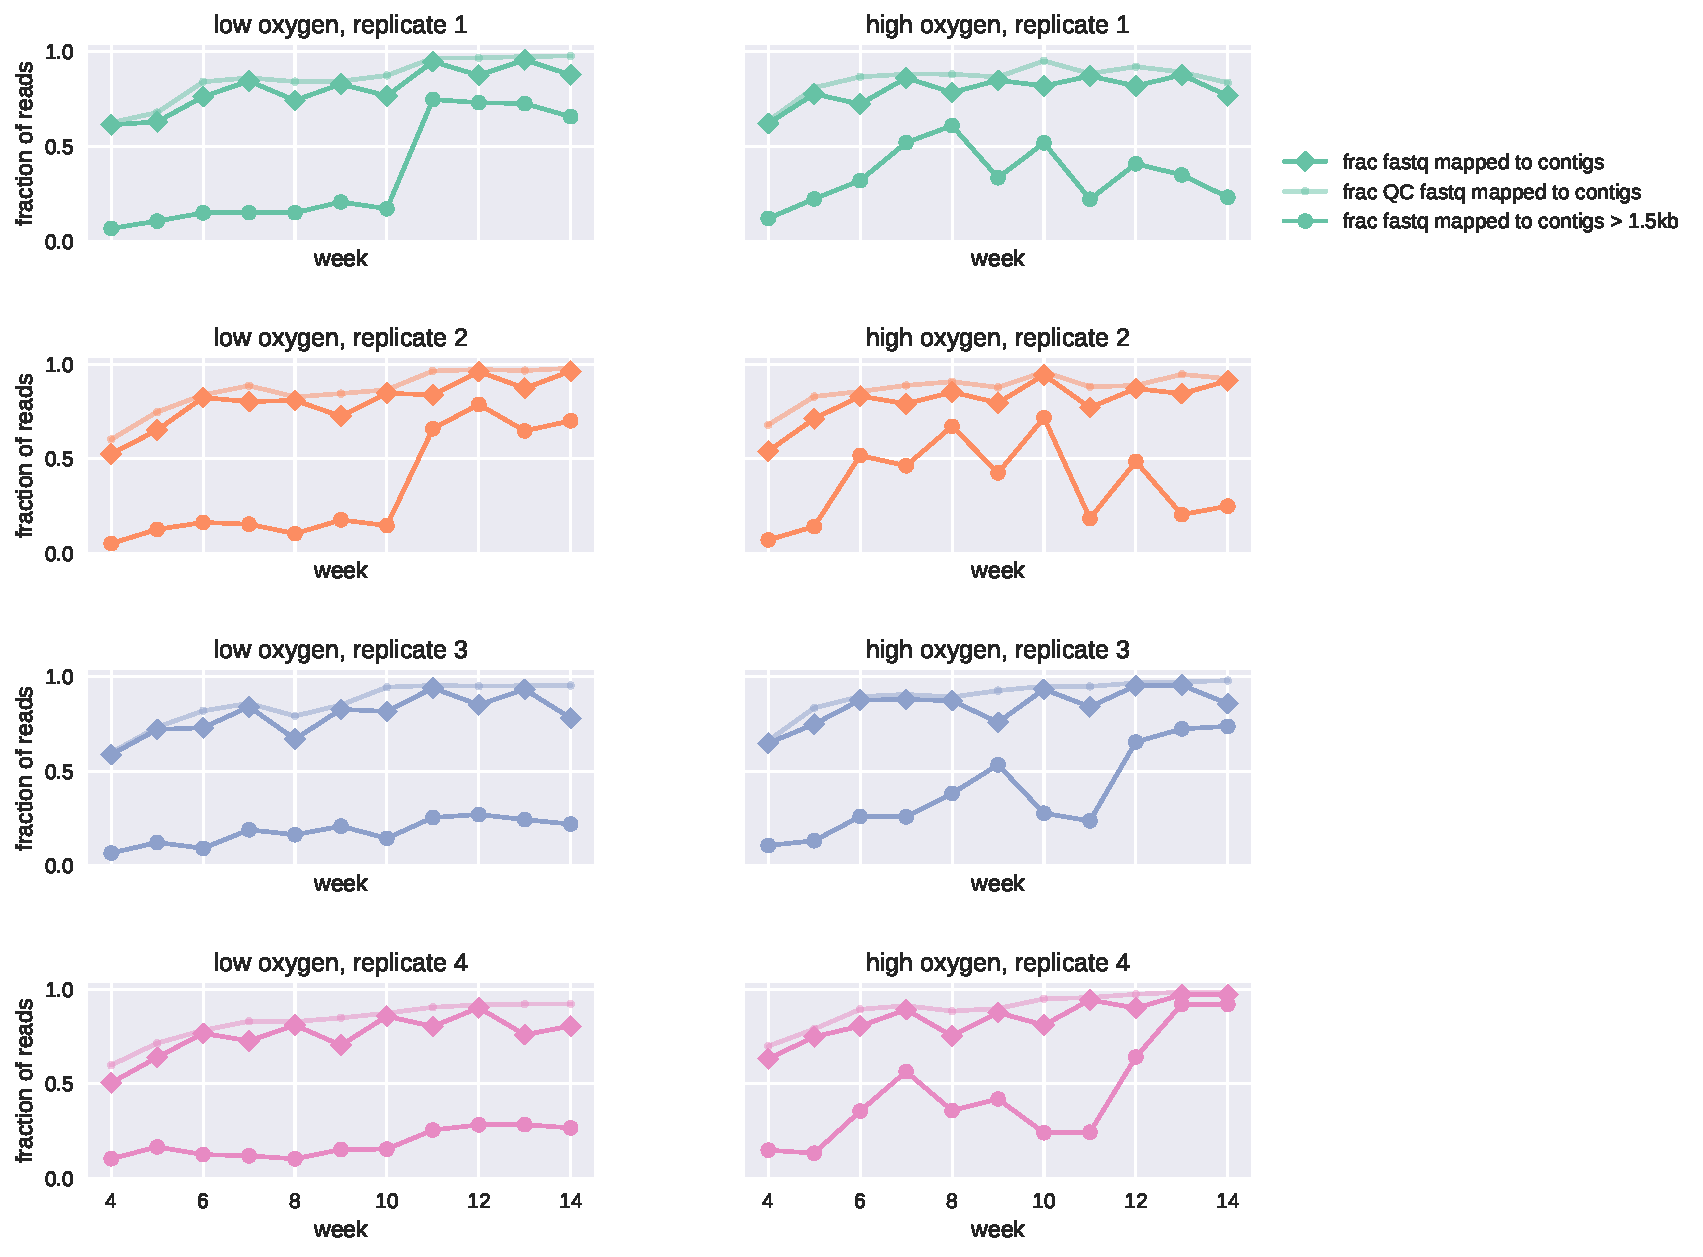
\includegraphics[width=1.0\textwidth]{./tex/chapter2/figures/170314_mapping_fractions--portrait.pdf}
    \begin{singlespace}
    \caption[Fraction of reads mapped to Elviz contigs]{
        Fraction of reads mapped to Elviz contigs.
        The top lines in each sub-plot show the fraction of reads that passed Elviz's QC filter.
        The diamond marks below indicate the fraction of total reads that mapped to contigs.
        The circle marks indicate the fraction that map to contigs with length $>$ 1.5kb, which are most promising for binning.
        }
    \label{fig:frac_elviz_mapped_to_contigs}
    \end{singlespace}
\end{figure}

\begin{singlespace}
\begin{longtable}{p{.50\textwidth} cc}
\caption[Highest expressed proteins, across samples]{
	The top 300 proteins when summing reads across the 88 samples.
    Sample size variation and gene length are not controlled for.
    See Table \ref{fig:frac_elviz_mapped_to_contigs} for sample size variation.} \\  % Need this \\  (http://tex.stackexchange.com/questions/148061/longtable-misplaced-noalign)
\label{table:top_genes} \\  % Need this \\  (http://tex.stackexchange.com/questions/148061/longtable-misplaced-noalign)
\toprule
                                           product & sum(RNA reads) & \# gene copies \\
\midrule \endfirsthead
% After \endfirsthead, repeat the labels again so they will appear on subsequent pages.
\toprule
                                           product & sum(RNA reads) & \# gene copies \\
\midrule

\endhead
\midrule
\multicolumn{3}{r}{{Continued on next page}} \\
\midrule
\endfoot

\bottomrule
\endlastfoot
\endlastfoot
                                                                      hypothetical protein &                 358,022,758 &       413,685 \\
                                 Particulate methane monooxygenase alpha subunit precursor &                 153,701,739 &            34 \\
                                  Ammonia monooxygenase/methane monooxygenase\%2C subunit C &                  87,810,398 &            38 \\
                                                                       Sensor protein ZraS &                  81,403,544 &           613 \\
                                            Particulate methane monooxygenase beta subunit &                  75,048,024 &            32 \\
                                                                                 Flagellin &                  12,453,840 &           155 \\
                                                                   Hydroxylamine reductase &                  11,249,260 &            13 \\
                                                                           S-layer protein &                   6,307,663 &             8 \\
                                                            Cell wall-associated hydrolase &                   5,121,957 &             8 \\
                                                                Capsid protein (F protein) &                   3,841,696 &             1 \\
                                 Methanol dehydrogenase [cytochrome c] subunit 2 precursor &                   3,405,479 &            27 \\
                                 Methanol dehydrogenase [cytochrome c] subunit 1 precursor &                   3,220,612 &            48 \\
                                                   ATP-dependent zinc metalloprotease FtsH &                   3,200,325 &           363 \\
                                                                Fimbrial protein precursor &                   3,181,026 &           638 \\
                                            Bacteriophage replication gene A protein (GPA) &                   2,954,718 &            49 \\
                                                      Microvirus H protein (pilot protein) &                   2,810,060 &             1 \\
                                                         Methane monooxygenase component C &                   2,769,830 &            30 \\
                                           Methanol dehydrogenase [cytochrome c] subunit 1 &                   2,751,386 &            69 \\
                                                      Group II intron-encoded protein LtrA &                   2,444,067 &           133 \\
                                                           3-hexulose-6-phosphate synthase &                   2,329,436 &            46 \\
                                                                           Transketolase 1 &                   2,312,198 &           123 \\
                                                                   PEP-CTERM motif protein &                   2,148,893 &           652 \\
                                                         Group 1 truncated hemoglobin GlbN &                   2,140,399 &           140 \\
                                                            Formaldehyde-activating enzyme &                   2,072,071 &           147 \\
                                                      Metal-binding protein SmbP precursor &                   2,064,649 &            77 \\
                                                                   Flp/Fap pilin component &                   2,014,075 &           100 \\
                                       ATP-dependent Clp protease ATP-binding subunit ClpA &                   1,907,981 &           121 \\
                                                               Flagellar hook protein FlgE &                   1,853,924 &           130 \\
                                                               DNA-binding protein HU-beta &                   1,689,620 &           176 \\
                                              Type II secretion system protein G precursor &                   1,659,638 &           384 \\
                                                       Flagellar hook-associated protein 2 &                   1,657,492 &           131 \\
                                                                         60 kDa chaperonin &                   1,621,356 &           167 \\
                                                                 Avirulence protein AvrBs3 &                   1,601,853 &             4 \\
                                                 DNA-directed RNA polymerase subunit beta' &                   1,586,236 &           152 \\
                                                                    Chaperone protein DnaK &                   1,544,707 &           277 \\
                                                    Methyl-accepting chemotaxis protein II &                   1,527,723 &           525 \\
                                                       Cyclic di-GMP phosphodiesterase Gmr &                   1,464,452 &         1,793 \\
                                                                     Elongation factor G 1 &                   1,453,588 &            38 \\
                                                          Phage Tail Collar Domain protein &                   1,434,560 &           159 \\
                                                           Major spike protein (G protein) &                   1,368,598 &             1 \\
                                                          Outer membrane porin F precursor &                   1,304,249 &           445 \\
                                           putative TonB-dependent receptor BfrD precursor &                   1,289,784 &           190 \\
                                                              Beta-lactamase TEM precursor &                   1,271,919 &             1 \\
                                                          3-hexulose-6-phosphate isomerase &                   1,232,120 &            48 \\
                                                             Phenol hydroxylase P5 protein &                   1,221,244 &            50 \\
                                                                              Lon protease &                   1,207,748 &           326 \\
                                                                       Aerobactin synthase &                   1,139,410 &            21 \\
                                                              Colicin I receptor precursor &                   1,124,515 &           439 \\
                                                                   Cold shock protein ScoF &                   1,123,655 &            52 \\
                                                              Cold shock-like protein CspA &                   1,117,436 &            40 \\
                                                             Phytochrome-like protein cph2 &                   1,105,919 &         1,558 \\
                                                                    putative peroxiredoxin &                   1,102,062 &            90 \\
                                                  DNA-directed RNA polymerase subunit beta &                   1,084,375 &           110 \\
                                                     Flagellar basal-body rod protein FlgG &                   1,076,811 &           128 \\
                               Bacterial extracellular solute-binding proteins\%2C family 3 &                   1,073,251 &           470 \\
                            Phenolphthiocerol synthesis polyketide synthase type I Pks15/1 &                   1,069,727 &            23 \\
                                                       Flagellar hook-associated protein 1 &                   1,060,718 &           116 \\
                                                                  30S ribosomal protein S1 &                   1,052,576 &           177 \\
                                                                   Chemotaxis protein CheA &                   1,049,177 &           280 \\
                                                     Flagellar basal-body rod protein FlgF &                   1,044,793 &            93 \\
                                                          RNA polymerase sigma factor RpoH &                   1,024,563 &           134 \\
                                   Cyclic di-GMP phosphodiesterase response regulator RpfG &                   1,009,170 &           931 \\
                                                                  Cytochrome c-L precursor &                   1,005,675 &            76 \\
                                                   Poly(beta-D-mannuronate) C5 epimerase 1 &                     984,141 &            17 \\
                                                     L\%2CD-transpeptidase catalytic domain &                     979,975 &           212 \\
                                                     Methyl-accepting chemotaxis protein I &                     976,610 &           309 \\
                                                                ATP synthase subunit alpha &                     960,915 &           147 \\
                                                                      Elongation factor Tu &                     958,727 &           140 \\
                                                                    Chaperone protein ClpB &                     942,491 &           211 \\
                                                              Right origin-binding protein &                     928,055 &            23 \\
                                                        Outer membrane protein A precursor &                     927,434 &           148 \\
                                       ATP-dependent Clp protease ATP-binding subunit ClpX &                     901,929 &           192 \\
                                                                   Chemotaxis protein CheY &                     897,095 &           430 \\
                                                           Modulator of FtsH protease YccA &                     892,776 &           137 \\
                                                                   Response regulator PleD &                     869,403 &           836 \\
                                                        putative CtpA-like serine protease &                     863,297 &           162 \\
                                                          RNA polymerase sigma factor RpoD &                     845,175 &           128 \\
                                                         Biopolymer transport protein ExbB &                     838,111 &           570 \\
                                                                        Spore protein SP21 &                     822,607 &           128 \\
                                        Polyketide cyclase / dehydrase and lipid transport &                     810,573 &           458 \\
                                Multidrug resistance outer membrane protein MdtP precursor &                     806,559 &           101 \\
                                                                             Protease HtpX &                     804,805 &           204 \\
                                                       Bacteriophage scaffolding protein D &                     794,345 &             1 \\
                                         Signal transduction histidine-protein kinase BarA &                     785,795 &           519 \\
                                                       preprotein translocase subunit SecY &                     779,178 &           134 \\
                                                                  50S ribosomal protein L2 &                     771,359 &           103 \\
                                                                 Superoxide dismutase [Fe] &                     764,292 &           138 \\
                                                   Transcriptional regulatory protein ZraR &                     759,073 &           845 \\
                                                           Putative deoxyribonuclease RhsC &                     754,966 &           161 \\
                                                                    Chaperone protein HtpG &                     748,660 &           188 \\
                                                            Minor curlin subunit precursor &                     748,058 &            12 \\
                                                                      Glutamine synthetase &                     746,921 &            91 \\
                                                                   Cold shock protein CspC &                     740,332 &            18 \\
                                                            Cytochrome c oxidase subunit 1 &                     740,292 &           171 \\
                                                        Outer membrane protein W precursor &                     727,458 &           117 \\
                                  putative phospholipid-binding lipoprotein MlaA precursor &                     726,741 &           195 \\
                                                                             Transaldolase &                     724,887 &           145 \\
                                                                  30S ribosomal protein S4 &                     716,789 &           141 \\
                                                                Cytochrome c-551 precursor &                     714,542 &           132 \\
                                                                 ATP synthase subunit beta &                     706,925 &           154 \\
                                                                Cell division protein FtsZ &                     682,952 &           157 \\
                                                     Ribosome hibernation promoting factor &                     672,173 &           122 \\
                                                           Modulator of FtsH protease HflK &                     670,892 &           239 \\
                                                                  30S ribosomal protein S2 &                     667,779 &           135 \\
                                                               Quercetin 2\%2C3-dioxygenase &                     662,723 &           414 \\
                                                     Peptidoglycan synthase FtsI precursor &                     655,407 &            39 \\
                                                            Transposase DDE domain protein &                     644,635 &           575 \\
                                                             Multidrug export protein EmrB &                     641,069 &           207 \\
                                                                 Ammonia channel precursor &                     638,801 &           258 \\
                                                                  Flagellar M-ring protein &                     637,658 &           112 \\
                                                                     ComE operon protein 1 &                     625,964 &            88 \\
                              putative periplasmic serine endoprotease DegP-like precursor &                     619,861 &           318 \\
                                                                      Cysteine desulfurase &                     617,548 &           464 \\
                                                  Cytochrome c oxidase subunit 2 precursor &                     617,471 &           138 \\
                                                            Cytochrome c oxidase subunit 3 &                     612,205 &           236 \\
                                                        Sporulation related domain protein &                     606,722 &           182 \\
                                                                  50S ribosomal protein L3 &                     598,078 &           111 \\
                                                          Nitrate/nitrite transporter NarK &                     598,069 &            62 \\
                                                        Flagellar P-ring protein precursor &                     596,197 &           113 \\
                                                 DNA-directed RNA polymerase subunit alpha &                     587,351 &           135 \\
                                                        Type II secretion system protein E &                     584,970 &           606 \\
                                                      Cytochrome c551 peroxidase precursor &                     581,414 &           306 \\
                                                     Copper resistance protein A precursor &                     579,604 &           174 \\
                                                                 50S ribosomal protein L25 &                     574,166 &           130 \\
                                                 Outer membrane porin protein 32 precursor &                     573,542 &           192 \\
                                                                    Flagellar protein FliT &                     549,417 &            30 \\
                                                                  50S ribosomal protein L1 &                     545,307 &           124 \\
                                               Respiratory nitrate reductase 1 alpha chain &                     543,710 &            45 \\
                                      Na(+)-translocating NADH-quinone reductase subunit F &                     540,161 &            44 \\
                                                      Linear gramicidin synthase subunit D &                     538,654 &            72 \\
                                         N-acetylmuramoyl-L-alanine amidase AmiC precursor &                     531,901 &           137 \\
                                                                              FecR protein &                     528,495 &           208 \\
                                                         Cation efflux system protein CusA &                     525,055 &           267 \\
                                                   Glucose-1-phosphate adenylyltransferase &                     519,029 &           150 \\
                                                                Hypoxic response protein 1 &                     514,246 &           168 \\
                                                            Putative formate dehydrogenase &                     514,121 &            67 \\
                                                   N\%2CN'-diacetylchitobiose phosphorylase &                     503,811 &            68 \\
                                                 Polyribonucleotide nucleotidyltransferase &                     501,398 &           142 \\
                                                          Ferrous iron transport protein B &                     497,854 &           158 \\
                                           Ribosomal RNA small subunit methyltransferase H &                     496,386 &           178 \\
                                               3-oxoacyl-[acyl-carrier-protein] synthase 1 &                     495,702 &           136 \\
                                                                            Trigger factor &                     495,625 &           132 \\
                                                                   TonB dependent receptor &                     489,761 &           770 \\
                                                          Copper-exporting P-type ATPase A &                     486,554 &           222 \\
                                  Membrane-bound lytic murein transglycosylase D precursor &                     485,735 &           279 \\
                                                                      Acyl carrier protein &                     475,902 &           248 \\
                                                   Flagellum site-determining protein YlxH &                     475,541 &            86 \\
                                        Bifunctional hemolysin/adenylate cyclase precursor &                     474,908 &           224 \\
                                                                 50S ribosomal protein L20 &                     472,974 &           117 \\
                                              Type II secretion system protein D precursor &                     466,040 &           360 \\
                                                                        Pyruvate kinase II &                     461,644 &           103 \\
                                                                               DNA primase &                     461,608 &           221 \\
                                                           Transposase IS66 family protein &                     458,000 &           220 \\
                                                        Ribose-phosphate pyrophosphokinase &                     454,049 &           201 \\
                                                       Flagellar biosynthesis protein FlhF &                     451,863 &            83 \\
                                                                 30S ribosomal protein S15 &                     450,754 &           121 \\
                                3-phenylpropionate/cinnamic acid dioxygenase subunit alpha &                     450,573 &            16 \\
                                                                   RNA-binding protein Hfq &                     444,771 &           107 \\
                                                                Maltodextrin phosphorylase &                     443,796 &           146 \\
                                       N(2)-citryl-N(6)-acetyl-N(6)-hydroxylysine synthase &                     440,152 &            15 \\
                           NAD(P)-dependent methylenetetrahydromethanopterin dehydrogenase &                     439,742 &           104 \\
                                                                  30S ribosomal protein S9 &                     438,650 &           142 \\
                                                         FeS cluster assembly protein SufB &                     436,043 &           110 \\
                            Type IV pilus biogenesis and competence protein PilQ precursor &                     427,396 &           224 \\
                                                 Ferredoxin-dependent glutamate synthase 1 &                     426,544 &            85 \\
                                                                 30S ribosomal protein S12 &                     423,584 &           101 \\
                                                 Osmotically-inducible protein Y precursor &                     422,220 &           304 \\
                                            ATP-dependent Clp protease proteolytic subunit &                     421,818 &           178 \\
                                                 Erythronolide synthase\%2C modules 1 and 2 &                     420,082 &             6 \\
                                                        Pyruvate-flavodoxin oxidoreductase &                     419,139 &            48 \\
                                         Fe(3+) dicitrate transport protein FecA precursor &                     418,819 &           132 \\
                                      Na(+)-translocating NADH-quinone reductase subunit B &                     417,928 &            28 \\
                                                    Glutamate synthase [NADPH] small chain &                     417,113 &           192 \\
                                                                cell division protein MraZ &                     415,859 &           129 \\
                                                       Flagellar hook-associated protein 3 &                     413,545 &            95 \\
                                                          Nitric oxide reductase subunit B &                     412,346 &           148 \\
                                                                2-isopropylmalate synthase &                     411,299 &           246 \\
                                                                     Aconitate hydratase 2 &                     410,938 &           109 \\
                                                                 50S ribosomal protein L27 &                     410,073 &           127 \\
                                                                  30S ribosomal protein S7 &                     409,297 &           104 \\
                                              Cyclic pyranopterin monophosphate synthase 1 &                     407,726 &            56 \\
                                                                          Bacterioferritin &                     406,109 &           166 \\
                                                                       Sensor protein FixL &                     405,443 &           475 \\
                                                               Dihydrolipoyl dehydrogenase &                     404,743 &           334 \\
                                                putative multidrug resistance protein EmrK &                     404,355 &            65 \\
                                                  Basal-body rod modification protein FlgD &                     404,309 &           107 \\
                                               3-oxoacyl-[acyl-carrier-protein] synthase 2 &                     403,698 &           435 \\
                   UDP-N-acetylmuramoyl-L-alanyl-D-glutamate--2\%2C6-diaminopimelate ligase &                     403,230 &           148 \\
                                                       preprotein translocase subunit SecA &                     400,638 &           232 \\
                                                                            Ribonuclease R &                     390,928 &           210 \\
                                                    Fructose-bisphosphate aldolase class 2 &                     389,633 &            63 \\
                                                                 50S ribosomal protein L10 &                     385,597 &           110 \\
                                                                      DNA translocase FtsK &                     384,995 &           152 \\
                                                            RNA polymerase sigma-54 factor &                     381,702 &           168 \\
                              UDP-3-O-[3-hydroxymyristoyl] N-acetylglucosamine deacetylase &                     379,042 &           171 \\
                                               Cobalt-zinc-cadmium resistance protein CzcA &                     376,307 &           608 \\
                                                           Modulator of FtsH protease HflC &                     373,571 &           135 \\
                                                       putative lipoprotein YiaD precursor &                     373,448 &           332 \\
                                                                Na(+)/H(+) antiporter NhaD &                     371,348 &           162 \\
                                                                  Squalene--hopene cyclase &                     366,723 &            41 \\
                                                                        Phosphoglucomutase &                     362,797 &           139 \\
                                              putative ABC transporter ATP-binding protein &                     362,766 &           553 \\
                                             Acetolactate synthase isozyme 3 large subunit &                     361,703 &            87 \\
                                                                       PilZ domain protein &                     361,543 &           389 \\
                                                              Phosphogluconate dehydratase &                     360,428 &           100 \\
                                                           FMN-dependent NADH-azoreductase &                     358,941 &            47 \\
                                                             Outer membrane efflux protein &                     355,020 &           711 \\
                                                         ECF RNA polymerase sigma-E factor &                     354,402 &           327 \\
                                                       Alpha/beta hydrolase family protein &                     354,213 &         1,330 \\
                                           3-oxoacyl-[acyl-carrier-protein] reductase FabG &                     353,830 &         1,263 \\
                                                       Pyruvate dehydrogenase E1 component &                     353,583 &           129 \\
                                                  NAD(P)H-quinone oxidoreductase chain 4 1 &                     353,001 &           102 \\
                                                                       Bacteriohemerythrin &                     352,386 &           136 \\
                             2\%2C3-bisphosphoglycerate-independent phosphoglycerate mutase &                     351,523 &           142 \\
                                      putative phospholipid-binding protein MlaC precursor &                     351,178 &           146 \\
                                           ATP:dephospho-CoA triphosphoribosyl transferase &                     350,953 &            54 \\
                                      Na(+)-translocating NADH-quinone reductase subunit C &                     350,710 &            24 \\
                                                                         DNA-invertase hin &                     350,432 &           272 \\
                                                               tol-pal system protein YbgF &                     349,970 &           181 \\
                                                     D-erythrose-4-phosphate dehydrogenase &                     347,666 &            22 \\
                                                    NADP-reducing hydrogenase subunit HndC &                     347,183 &            84 \\
                                                                         10 kDa chaperonin &                     347,019 &           113 \\
                                                                 6-phosphogluconolactonase &                     344,336 &           284 \\
                                              Peptidase propeptide and YPEB domain protein &                     344,261 &           141 \\
                                                                   Chemotaxis protein CheW &                     344,064 &           326 \\
                                            Succinyl-CoA ligase [ADP-forming] subunit beta &                     343,575 &           175 \\
                                                  Carbamoyl-phosphate synthase large chain &                     341,882 &           188 \\
                                                                  Polyketide synthase PksN &                     341,165 &             7 \\
                      putative parvulin-type peptidyl-prolyl cis-trans isomerase precursor &                     340,103 &           132 \\
                                                     Flagellar hook-length control protein &                     339,156 &            56 \\
                                                          Methyltransferase domain protein &                     338,398 &           367 \\
                                               NAD-reducing hydrogenase HoxS subunit alpha &                     338,348 &            38 \\
                                                    Inosine-5'-monophosphate dehydrogenase &                     337,284 &           207 \\
                                                                    flagellar protein FlaG &                     335,036 &            64 \\
                                                              Glycosyl hydrolase family 57 &                     334,643 &            60 \\
                                                                  50S ribosomal protein L4 &                     333,085 &           111 \\
                           ATPase family associated with various cellular activities (AAA) &                     332,936 &           296 \\
                                                Phosphoribosylformylglycinamidine synthase &                     331,827 &           142 \\
                                                        Rod shape-determining protein MreB &                     331,122 &           173 \\
                                                                   Response regulator UvrY &                     329,883 &           400 \\
                                                       Signal recognition particle protein &                     329,618 &           149 \\
                                                          Tetratricopeptide repeat protein &                     329,174 &         1,427 \\
                                                      Thermostable monoacylglycerol lipase &                     327,977 &            55 \\
                                                                  30S ribosomal protein S3 &                     326,369 &            93 \\
                                                                 Tim44-like domain protein &                     322,952 &           105 \\
                                         Oxygen-independent coproporphyrinogen-III oxidase &                     320,953 &           201 \\
                                                                    ATP synthase subunit c &                     320,002 &           136 \\
                                                                 50S ribosomal protein L15 &                     319,012 &           116 \\
                                                          RNA polymerase sigma factor SigA &                     317,688 &            83 \\
                                                                              FlgN protein &                     316,776 &            63 \\
                                                       Ferrichrome receptor FcuA precursor &                     315,542 &            88 \\
                                                                       HDOD domain protein &                     313,422 &           460 \\
                                                            dTDP-glucose 4\%2C6-dehydratase &                     312,803 &           341 \\
                                                       Flagellar motor switch protein FliM &                     312,289 &           104 \\
                                                                ATP synthase subunit delta &                     312,084 &           107 \\
                                                          tetratricopeptide repeat protein &                     311,426 &           444 \\
                                                 N\%2CN'-diacetyllegionaminic acid synthase &                     310,503 &            95 \\
                                                                   Formate dehydrogenase H &                     310,054 &            94 \\
 Dihydrolipoyllysine-residue acetyltransferase component of pyruvate dehydrogenase complex &                     309,903 &           254 \\
                                                                       MOSC domain protein &                     308,478 &           104 \\
                                      Na(+)-translocating NADH-quinone reductase subunit D &                     308,303 &            20 \\
                                                                 50S ribosomal protein L14 &                     307,247 &           110 \\
                                                                               Transposase &                     307,033 &           581 \\
                                                           Chaperone protein Skp precursor &                     305,658 &           115 \\
                                UDP-N-acetylmuramoyl-tripeptide--D-alanyl-D-alanine ligase &                     304,306 &           183 \\
                                                      Septum site-determining protein MinD &                     302,251 &           202 \\
                                                                 Tyrosine recombinase XerC &                     302,003 &           607 \\
                                                                      Malate dehydrogenase &                     301,547 &           151 \\
                                                                  50S ribosomal protein L6 &                     300,590 &           120 \\
                                                                ATP synthase epsilon chain &                     300,575 &           150 \\
                                                                  50S ribosomal protein L5 &                     299,638 &           112 \\
                                                                    transport protein TonB &                     299,458 &           222 \\
                                                                    Adenosylhomocysteinase &                     299,382 &           173 \\
                                                                    Chaperone protein DnaJ &                     298,386 &           374 \\
                                                                 50S ribosomal protein L17 &                     296,464 &           143 \\
                                                              50S ribosomal protein L7/L12 &                     295,549 &           122 \\
                                                                Dihydroxy-acid dehydratase &                     295,169 &           189 \\
                                           ATP-dependent Clp protease adapter protein ClpS &                     294,553 &           112 \\
                                                                       Multicopper oxidase &                     294,469 &            44 \\
                                                 UDP-3-O-acylglucosamine N-acyltransferase &                     294,322 &           188 \\
                                                        Type II secretion system protein F &                     293,302 &           371 \\
                                         Phospho-N-acetylmuramoyl-pentapeptide-transferase &                     292,626 &           171 \\
                                                                  30S ribosomal protein S5 &                     291,627 &           114 \\
                                                     L-2\%2C4-diaminobutyrate decarboxylase &                     291,090 &            57 \\
                                                                  anti-sigma28 factor FlgM &                     290,901 &            71 \\
                                                          Phytanoyl-CoA dioxygenase (PhyH) &                     289,636 &           142 \\
                                                                 30S ribosomal protein S13 &                     289,348 &           109 \\
                                                                    Threonine--tRNA ligase &                     288,502 &           120 \\
                                                Iron-sulfur cluster insertion protein ErpA &                     287,287 &           204 \\
                                                                      NAD(P)H azoreductase &                     286,417 &            65 \\
                                                       Flagellar biosynthesis protein FlhA &                     285,954 &           101 \\
                                   Nicotinate-nucleotide pyrophosphorylase [carboxylating] &                     284,572 &           144 \\
                                                   Poly(beta-D-mannuronate) C5 epimerase 5 &                     283,725 &            25 \\
                                                                  ATP synthase gamma chain &                     283,576 &           137 \\
                                              Outer membrane efflux protein BepC precursor &                     282,205 &           131 \\
                                                    Molybdenum-pterin-binding protein MopA &                     281,225 &           168 \\
                                                                      Cupin domain protein &                     277,550 &           631 \\
                            Chemotaxis response regulator protein-glutamate methylesterase &                     276,474 &           192 \\
                                              UTP--glucose-1-phosphate uridylyltransferase &                     275,652 &           143 \\
                                                        putative FAD-linked oxidoreductase &                     275,649 &           382 \\
\end{longtable}
\end{singlespace}



\begin{figure}[H]
\centering
    % /Users/janet/Dropbox/meta4_bins_data_and_files/170124_current_metabat_analysis_figures/170124_bad_low_o2_samples_have_more_reads_on_short_contigs--binning_not_considered.pdf
    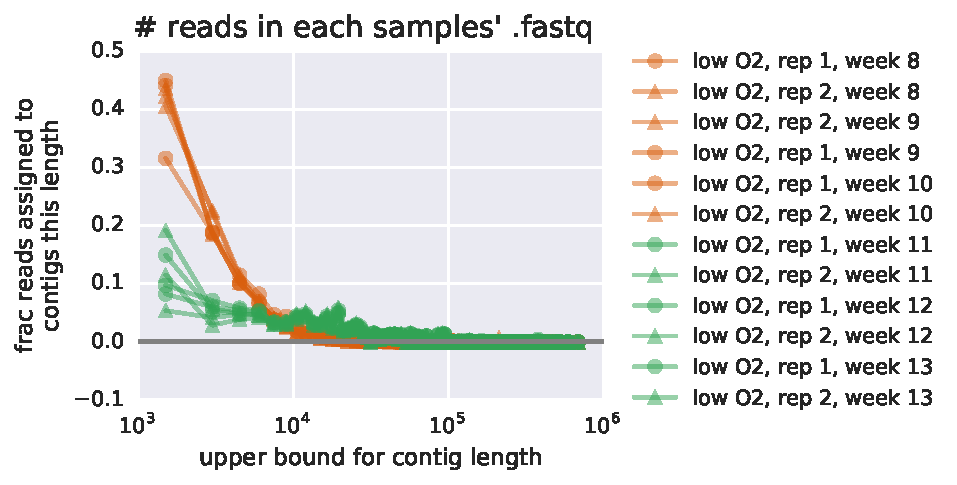
\includegraphics[width=1.0\textwidth]{./tex/chapter2/figures/170124_bad_low_o2_samples_have_more_reads_on_short_contigs--binning_not_considered.pdf}
    \begin{singlespace}
    \caption[Samples best explained by bins have more reads drawn to longer contigs]{
        Samples with metagenomes that are well represented by MetaBAT bins have more reads drawn to longer contigs.}
    \label{fig:contig_dist}
    \end{singlespace}
\end{figure}



